% !TeX root = ../main.tex
\chapter[Evaluating and Improving Testing For Memory Consistency Specifications]{Evaluating and Improving Testing For Memory Consistency Specifications}
\label{chap:mc_mutants}

\newcommand{\sys}{MC Mutants\xspace}

\section{Personal Context}

\newcommand{\corrlitmustest}{
    \begin{tabular}{l l}
    \midrule
    \underline{thread 0} & \underline{thread 1} \\
        \circledBlack{\vphantom{A}a}\hspace{.1cm} \texttt{v0 = atomicLoad(x)} &  \circledWhite{\vphantom{A}c}\hspace{.1cm} \texttt{atomicStore(x,1)}  \\
        \circledBlack{\vphantom{A}b}\hspace{.1cm} \texttt{v1 = atomicLoad(x)} &  \\
        \midrule
        \multicolumn{2}{c}{Condition: \texttt{v0 == 1 \&\& v1 == 0}}
    \end{tabular} \hspace{1cm}
}

\newcommand{\mprelacqlitmustest}{
    \begin{tabular}{l l}
    \midrule
    \underline{thread 0} & \underline{thread 1} \\
        \circledBlack{\vphantom{A}a}\hspace{.1cm} \texttt{atomicStore(data, 1)} &  \circledWhite{\vphantom{A}d}\hspace{.1cm} \texttt{r0 = atomicLoad(flag)}  \\
        \circledBlack{\vphantom{A}b}\hspace{.1cm} \texttt{fence(release)} &  \circledWhite{\vphantom{A}e}\hspace{.1cm} \texttt{fence(acquire)}  \\
        \circledBlack{\vphantom{A}c}\hspace{.1cm} \texttt{atomicStore(flag, 1)} &
        \circledWhite{\vphantom{A}f}\hspace{.1cm} \texttt{r1 = atomicLoad(data)}  \\
        \midrule
        \multicolumn{2}{c}{Condition: \texttt{r0 == 1 \&\& r1 == 0}}
    \end{tabular} \hspace{1cm}
}

\begin{figure}
\centering
\small
\captionsetup[subfigure]{width=.7\columnwidth}
\subfloat[Coherence of Read-Read (CoRR) litmus test]{\corrlitmustest \label{fig:CoRR-executable}} \\
\subfloat[Message Passing rel/acq (MP-relacq) litmus test]{\mprelacqlitmustest \label{fig:MP-executable}}
\caption{Two litmus tests that illustrate bugs in WebGPU found by our work.  We observed executions that resulted in the condition being true, even though it is disallowed by the MCS. All memory is initialized to 0.}
\label{fig:litmus-executables}
\end{figure}

\begin{figure}
\centering
    \subfloat[Disallowed execution of the CoRR litmus test]{{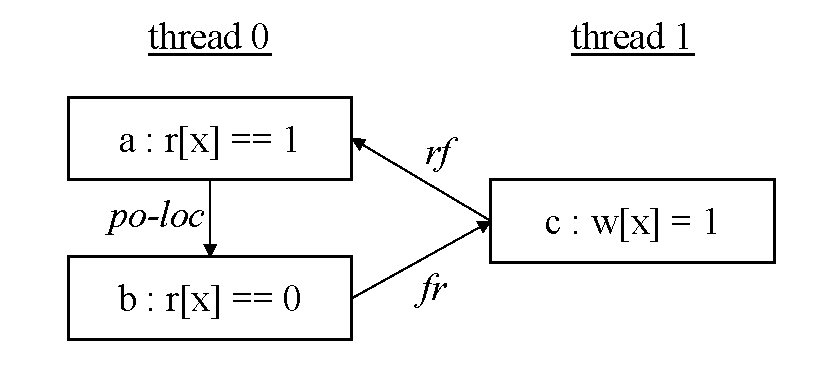
\includegraphics[width=0.6\columnwidth]{images/CORR.pdf} \label{fig:litmus:CoRR}}} \\
    \subfloat[Disallowed execution of the MP-relacq litmus test]{{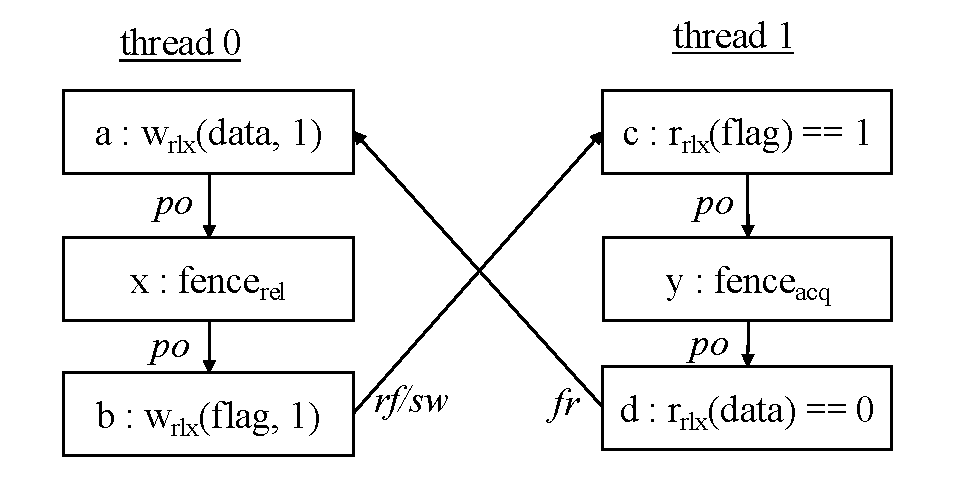
\includegraphics[width=0.6\columnwidth]{images/mp-relacq.pdf} \label{fig:litmus:MP-relacq}}}
    \caption{Candidate executions for the litmus tests shown in \myfig\ref{fig:litmus-executables} illustrating behaviors disallowed by the WebGPU MCS.}
    \label{fig:litmus-examples}
\end{figure}

\section{Motivation}

A memory consistency specification (MCS) for a shared memory runtime platform  defines the legal values that loads are allowed to observe, and thus, is crucial for program reasoning.  For efficiency reasons~\cite{mem-model-performance}, many platforms provide a \textit{relaxed} MCS, which allows complex behaviors. Validating that a platform implementation honors its MCS is a difficult, yet important, since a bug may lead to rare, non-deterministic application errors~\cite{pldi16,program-transforms}.

Early MCS testing work executed sequences of memory accesses~\cite{archtest, tsostore} and then analyzed a trace of the observed values.  More recent work uses formal specifications to derive small concurrent tests, often called \textit{litmus tests}, which are then executed for many iterations, checking for a violation at each iteration~\cite{litmus}. Litmus testing strategies have found numerous bugs in runtime platforms~\cite{oopsla2020,asplos15,power-bug,rtl-check, fences}.

\subsection{Motivating Examples \label{sec:motivating-examples}}
The effectiveness of litmus testing approaches is \textit{extremely} sensitive to the testing environment, i.e.\ the context around the litmus test that creates stress on the platform. We use the two litmus tests of \myfig\ref{fig:litmus-executables} to illustrate this.
%
The CoRR (Coherence of Read-Read) test, shown in \myfig\ref{fig:CoRR-executable}, tests if the first read in a thread (operation \circledBlack{a}) can observe an updated value (from operation \circledWhite{c}), while a following read (operation \circledBlack{b}) reads a stale value (from the initial state).  A straightforward testing environment (i.e.\ one without stress) observes no violations, but when executed in a stressful testing environment (e.g.\ as used in ~\cite{asplos15,oopsla2020}), the test evinces a bug in the WebGPU platform when executing on an Apple device with an Intel GPU.\footnote{The bug is in the WebGPU implementation, whereby Google Chrome layers over Apple's platform-level Metal API. We have filed an issue with Apple and await a resolution.}

The MP-relacq (Message Passing relacq) litmus test, shown in \myfig\ref{fig:MP-executable}, writes to location \texttt{x} (\circledBlack{a}) and sets a flag (\circledBlack{c}) in thread 0, then reads the flag (\circledWhite{d}) and reads the data (\circledWhite{f}) in thread 1.  The fence instructions synchronize across the threads. A violation occurs if thread 1 observes the updated flag without observing the updated data.  While existing stress testing environments did not reveal any violations, our novel parallel approach was able to observe violations in the WebGPU platform on AMD GPUs. This resulted in a
fix to an AMD Vulkan compiler and a specification change to the WebGPU MCS~\cite{webgpu-spec-change}.

When testing, it is impossible to tell if an unobserved illegal execution is not allowed or if it is simply rare and was not exposed by the tests.  Thus, effective MCS testing requires tuning testing environments to reduce the possibility of a missed bug.  However, legitimate MCS violations are exceeding rare, and thus cannot be used as a metric for such tuning efforts.  Existing approaches have tuned their testing environments by maximizing the number of weak, but allowed, behaviors of some litmus tests, yet have not provided justification on why this metric is valid.  Finally, existing MCS testing techniques do not provide confidence in their ability to find MCS bugs.  Consequently, it is difficult to gauge whether it is worth the time to perform more testing, especially when running in time-constrained environments such as a conformance test suite.  The result of these limitations has been a lack of adoption of existing MCS testing approaches.

\subsection{Our Approach: \sys \label{sec:our-approach}}

In this work, we propose \textit{Memory Consistency Mutants} or \sys, a methodology that quantitatively evaluates MCS testing environments using black-box mutation testing~\cite{black-box,mutation-testing}. Litmus tests are \textit{mutated} in such a way that the erroneous behavior that the test was checking is are now allowed.  A test environment \textit{kills} the mutated test (mutant) by observing the newly allowed execution. The number of mutants that are killed is called the \textit{mutation score}. Additionally, \sys can be used to record the speed at which the mutants are killed, called the \textit{mutant death rate}.

Intuitively, mutants check for an allowed weak memory or fine-grained interleaving  behavior that is closely related to a disallowed behavior of an MCS litmus test. Our main contribution arises in formally defining this notion of \textit{related}; \sys generates mutants systematically by disrupting edges in a happens-before cycle of a disallowed behavior, corresponding to a small change in the program syntax of the litmus test.

The effectiveness of a testing environment can be evaluated by its mutation score (and mutant death rate) when executing mutants. Thus, a test environment must aim to maximize legal behavior in the mutants that closely relates to the illegal behavior in the original litmus tests. Hence, there are two constraints upon which \sys depends.

First, the legal mutant behavior must be \textit{observable} on the testing platform. That is, even if the mutant behavior is allowed by the specification, it may not be observable on the testing platform. If the mutant behavior is not observable, then \sys will be unable to evaluate the testing environment with respect to the given mutant and corresponding litmus test. Our results (see \mysec\ref{sec:mut-scores}) show that most mutant behavior is observable on GPUs across a range of mainstream vendors.  However, this might not hold for all platforms, or mutants, in which case the mutants should be pruned according to the expected observable behavior on the implementation (discussed more in \mysec\ref{sec:observed-mutants}).

Second, the validity of \sys depends on a correlation between observing legal mutant behavior and real MCS bugs.  We validate this correlation by showing that a testing environment's ability to kill a mutant is highly correlated with its ability to find related MCS bugs in three cases (\mysec\ref{sec:corr-analysis}).  This also means that testing environments that do not reliably kill mutants are not able to expose the MCS bugs.


%\newtext{If the mutant is killed with a high degree of reproducibility during test runs, then a bug corresponding to that mutant should be easily observed when running the non-mutated conformance test. If the bug is not observed, then we can say with high probability that the illegal execution is impossible (i.e. there is no bug).} \rl{improve motivation (reviewer B)} \arq{This is highly redundant with the next paragraph.  Note to self--Come back and fix}

%Thus, these mutations aim to model implementation bugs that fail to enforce a happens-before relation in an execution




\sys enables principled evaluation and optimization of MCS test environments.  An optimized testing environment can increase the confidence that MCS bugs will be found, if they exist, using the original, un-mutated test suite. We utilize \sys to develop two novel testing environment improvements: a parallel testing environment and a testing confidence strategy. Using a combination of these contributions, we show that both bugs we identified in \myfig\ref{fig:litmus-executables} are rapidly and reliably revealed in testing environments optimized using \sys. We now detail our testing environment contributions.

%In this paper, we use \sys to help us develop and evaluate two additional contributions to litmus test environments: parallel testing and a testing confidence strategy.

\paragraph{Parallel Testing Environment (PTE)}
While previous work ran litmus tests in parallel on multicore CPUs~\cite{litmus}, the effectiveness was limited by the low number of cores found on traditional SMP CPU machines.
%and took advantage of independent thread execution.
As the number of parallel tests increases, it becomes difficult to scale thread-to-test assignment in a way that is safe, efficient, and effective; especially in the presence of tunable stress parameters. Given this, prior techniques for running parallel litmus tests do not generalize to GPUs.
%due to issues such as the sensitivity of SIMT execution, overhead in ensuring parallel tests do not lead to memory conflicts, and balancing execution of testing and stressing threads.}

We overcome these challenges with a novel parallel testing technique that uses a parallel permutation strategy based on modular arithmetic of co-prime numbers to assign test instances to threads with low overhead.
%and no divergent control flow.
This approach, which we call \textit{Parallel Testing Environments}, or PTE, allows us to increase mutant death rates by on average three orders of magnitude over previous work.
%
%\oldtext{First, we develop a novel technique that executes many litmus test instances in parallel, known as the \textit{Parallel Testing Enivornment} or PTE. This approach is especially useful on many-core systems, like GPUs, which can execute many threads in parallel. We use \sys to show that a GPU implementation of PTE increases the mutant death rate by three orders of magnitude, on average.}
Moreover, \sys shows that parallel testing synergizes with the stress testing environment given in prior work~\cite{oopsla2020}, which increases the mutant death rate by an additional 43\%.
%
The efficiency gained using PTE is critical for observing the MP-relacq bug (\myfig\ref{fig:MP-executable}). We were unable to observe it through extensive stress tuning using techniques from prior work. However, under PTE, it readily appears at a rate of 10.4 violations per second.
%with no added stress, at a rate of .81 violations per second. If the testing environment is further tuned using \sys, the rate increases to 10.4 per second.

\paragraph{MCS Test Confidence}

It is impossible to have complete confidence that testing will uncover bugs, as litmus tests are non-deterministic. However, we can utilize \sys to provide a \textit{reproducibility score} for a testing environment.  This is a statistical confidence that a testing run will kill a mutant given the mutant death rate on previous runs.  It is parameterized by a time budget, i.e.\ how long each test can be run for. %The reproducibility score can also be used to combine test environments while maximizing the number of tests that meet some required confidence level.
Our results, across four GPUs spanning four mainstream vendors, that on our tuned parallel test environment can provide a mutation score of 82\% and a reproducibility score of 99.999\% with a budget of 64 seconds per test, %\oldtext{meeting a level of reliability commonly considered an industry standard~\cite{carrier-grade}. Additionally, the parallel environments can match}
matching the maximum mutation score achieved by prior work with $(1/4096)^{\text{th}}$ the time budget. Reproducibility scores provide a principled way to evaluate the relative effectiveness of test environments at finding bugs.
%Additionally, the reproducibility score minimizes loss as time budgets are reduced, achieving a mutation score of 75.8\% for the same reproducibility target and a time budget of only 1 second per test.

\paragraph{Evaluation Specification} We evaluate our approach
%\sys, parallel testing environments, and MCS test confidence
in WebGPU \cite{webgpu}, a new web-based \textit{general purpose} GPU (GPGPU) framework. WebGPU has a hierarchical execution model similar to other GPU platforms, e.g.\ CUDA and OpenCL. Threads are partitioned into workgroups, and there are several different memory regions.

%WebGPU is a high-level framework designed to execute on GPUs produced by a diverse set of chip vendors, each of which produce their own GPU that has its own unique MCS.
%As WebGPU's MCS differs from any individual hardware MCS, our testing strategy focuses on the abstraction WebGPU provides, while remaining general enough to be applied to any MCS in the future (see \mysec\ref{sec:webgpu} for details).
%
%WebGPU differs from other specifications in that it targets devices from a wide range of vendors, e.g., Intel, AMD, Apple, and Nvidia (with mobile devices in the near-future road map). In fact, WebGPU targets the widest
%
%WebGPU sets itself apart from other frameworks by targeting the widest range of GPU devices for any GPU platform with an MCS. This ambitious
%
However, the WebGPU MCS differs from other specifications in that it targets devices from a wide range of vendors, e.g., Intel, AMD, Apple, and NVIDIA.\footnote{With mobile support planned in the future, this will include even more vendors, e.g.\ Qualcomm, ARM and Imagination.} In fact, it has the \textit{largest} set of backends targeted by any GPGPU MCS. To provide a portable abstraction across these devices, WebGPU currently has relatively few options for synchronization; there are no sequentially consistent atomic operations as seen in NVIDIA's PTX~\cite{ptx-memory-model}, or OpenCL~\cite{sc-in-opencl}. However, the few ordering properties that WebGPU provides, such as coherency across atomic accesses, must be preserved across all devices. Given this unique context, MCS testing is both \textit{critical}, as it must ensure a single consistent MCS on a diverse set of backends, and \textit{challenging}, as testing environments must be effective across many devices.
%

This work targets only one level (or \textit{scope}) of the GPU execution hierarchy, specifically threads that are in different workgroups. We pick this scope for three reasons: (1)~it is pragmatic, as there is no other way for inter-workgroup threads to communicate without the expensive routine of stopping and relaunching the kernel, (2)~prior work developed stress techniques targeting this scope~\cite{oopsla2020}, providing testing environments that we can tune and evaluate, and (3)~WebGPU does not (yet) expose the subgroup (or warp in CUDA) scope, and thus it cannot be tested. However, \sys applies generally to MCS testing, and we aim to apply it to the more complete GPU execution hierarchy as the specification, stress testing techniques, and application use-cases continue to evolve.

%
% it is extremely challenging to ensure ordering properties are preserved across each backend; and as such,
%
%To account for the diversity of devices, the current abstractions provide very few ordering properties.
%As a consequence, there are very few ordering properties available in the current iteration of the framework; however, these ordering properties must be implemented correctly across a broader range of devices

%As a consequence, MCS testing is particularly critical

%As a consequence, there are currently very few ordering guarantees in the language  to induce synchronization between threads, e.g., through fence instructions; see \mysec\ref{sec:background}
%
%MCS testing is particularly challenging for platforms like WebGPU, as different devices require different testing environments to be effective~\cite{oopsla2020}.
%
%As such, WebGPU is an ideal framework to develop portable and robust testing methodologies, as we propose in this work.



Using \sys, a set of 20 litmus tests and 32 mutant tests were created. We evaluate these tests across four GPU devices, spanning four vendors: Apple, AMD, Intel, and NVIDIA, for a total of 128 mutant/device combinations. One major impact of this work is its adoption into the WebGPU conformance test suite (CTS)  for testing the MCS (see \mysec\ref{sec:impact}).
%The tuned parallel testing strategy, kills 83.5\% of mutants, an 81.4\% increase over the strategies used by prior work, with the average mutant death rate is $2731\times$ higher than prior work.




\subsection{Contributions}

\paragraph{Contributions} In summary, our contributions are:
\begin{enumerate}
    \item \sys: A mutation testing approach that can evaluate MCS testing environments (\mysec\ref{sec:mc-mutants}).
    \item A novel parallel test environment that executes litmus test instances in parallel (\mysec\ref{sec:parallel-tests}).
    \item An MCS test confidence strategy using a reproducibility score parameterized over a time budget (\mysec\ref{sec:rep-heuristic}).
    \item An \sys implementation and evaluation in WebGPU. Our evaluation spans 4 different GPUs from 4 different vendors and shows that: (\mysec\ref{sec:evaluation})
    \begin{itemize}
        \item \sys generates a test suite consisting of 20 un-mutated litmus tests and 32 mutated litmus tests.
        \item parallel testing environments are able to kill 81\% more mutants with an average mutant death rate over $2000\times$ higher than prior work.
        \item our MCS test confidence can explore trade-offs in reproducibility and time for test engineering.
    \end{itemize}
\end{enumerate}

%\noindent
We highlight two impacts of this work: first, it identified two MCS bugs in WebGPU implementations, one of which led to a specification change.  Second, the work has been adopted into
the WebGPU CTS (\mysec\ref{sec:impact}). The effectiveness of parallel test environments was a critical factor in getting the tests added to the CTS, as the full CTS must be run often during development. The strategies we developed for evaluating MCS test confidence allowed us to propose a time budget of approximately one minute on average desktop hardware for the full MCS test suite, adding little overhead to the full CTS.


\begin{figure}
\centering
\subfloat[3-event reversing \textit{po-loc} mutator]{{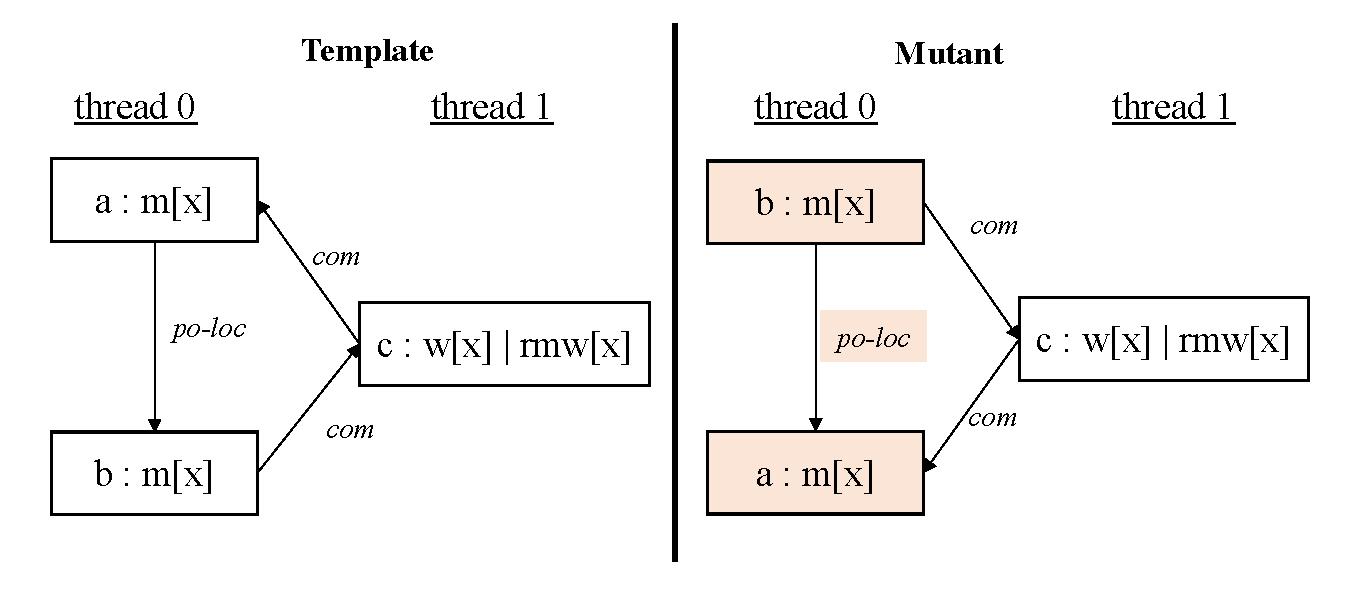
\includegraphics[width=0.8\columnwidth]{images/mutator1.pdf}\label{fig:mutator-1}}} \\
\subfloat[4-event weakening \textit{po-loc} mutator]{{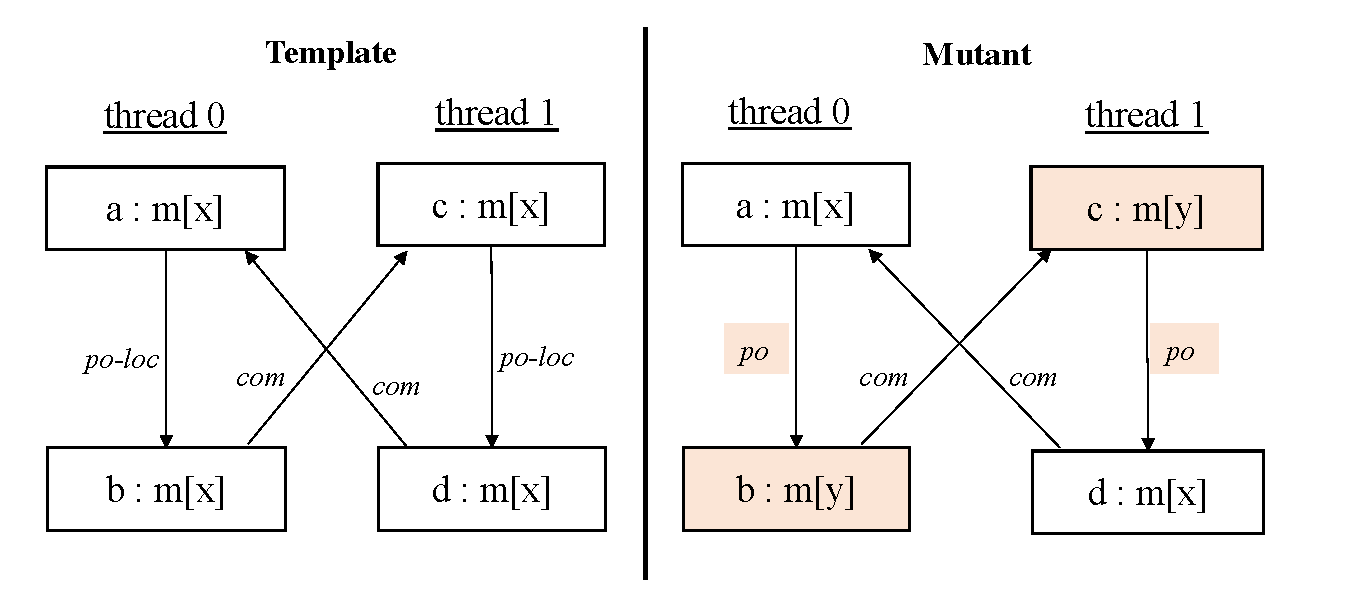
\includegraphics[width=0.8\columnwidth]{images/mutator2.pdf}\label{fig:mutator-2}}} \\
\subfloat[4-event weakening \textit{sw} mutator]{{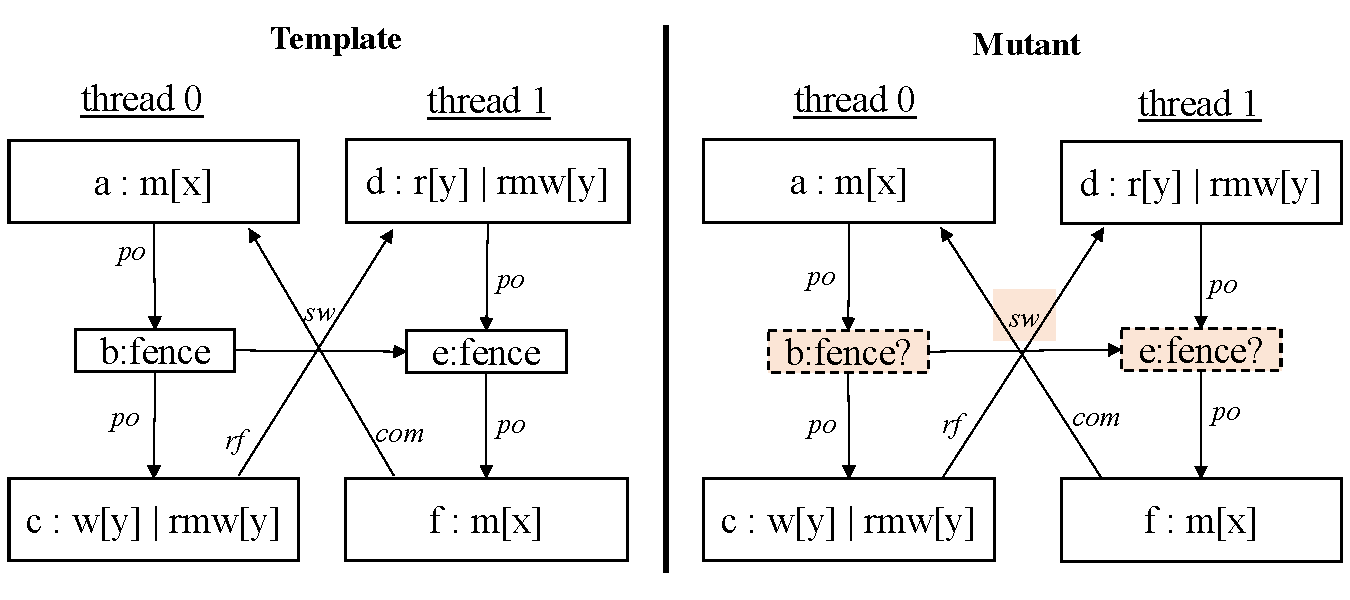
\includegraphics[width=0.8\columnwidth]{images/mutator3.pdf}\label{fig:mutator-3}}}
\caption{The three cycles used to instantiate conformance tests and mutants, with conformance test templates shown on the left and mutant templates on the right; \textit{m[x]} signifies an abstract memory event which may be instantiated as a read, write, or RMW. The disrupted events and edges are highlighted in red. \label{fig:mutators}}
\end{figure}

\section{MC Mutants}

\sys is a methodology for evaluating MCS testing environments. This approach uses cyclic candidate executions from litmus tests, as described in \mysec\ref{sec:litmus-tests}. The methodology then mutates cyclic executions by disrupting one of the edges and generates mutated test programs by reconstructing the instructions that led to the execution. The mutated test now has an execution that is allowed by the MCS, but is closely related to a behavior that is disallowed by the MCS.

In order to ensure that mutant programs can be reconstructed from the mutant execution, the mutation process focuses on disrupting relations that correspond to the \textit{syntax} of the program, as opposed to relations that arise dynamically. For example, the \textit{po} relation arises from the program syntax, i.e.\ the order of instructions in the test. Similarly, the \textit{sw} relation arises from fence instructions in the program syntax. This is important for our black-box mutation approach, as our only interface to the platform is with programs (and their syntax). Thus, our mutations encode modifications that we can actually implement. The behaviors allowed under the mutated test are behaviors that will appear in the original test if there is a bug in the implementation of the MCS, since the MCS restricts correct executions to \textit{not} disrupt these relations.

%\oldtext{The edge disruptions performed by the mutations aim to correspond to errors that may occur in implementations. Thus, a testing environment that is able to observe mutant behaviors should also be able to catch actual implementation errors when run on the non-mutated set of tests. Additionally, the rate at which a testing environment observes mutant behaviors can be used to reason about how many iterations a non-mutated test should be run in order to have confidence that it would catch an implementation bug corresponding to a mutated test.}

MC Mutants uses a set of \textit{mutator} functions and a function that converts executions into programs. A mutator consist of an abstract happens-before cycle $T$ (similar to those from Alglave et al.~\cite{fences}) and an edge disruptor process $E$. The mutator returns $L$, a set of \textit{conformance} litmus tests that contain disallowed candidate executions based on $T$, and $M$, a set of mutated tests containing candidate executions (closely related to the disallowed behaviors in $L$) for which the behavior is now allowed. A testing environment can be evaluated as follows; the ability of a testing environment to kill (i.e. observe) mutants in $M$ corresponds to its ability to observe an implementation error corresponding to $E$ when running $L$.


This paper describes three distinct mutators, summarized in \myfig\ref{fig:mutators}. Each mutator enumerates all possible syntactic edge disruptions, i.e.\ $po$, $sw$, and $\textit{po-loc}$, and can be seen as a complete set of mutants for these abstract happens-before cycle templates. Overall, there are 20 conformance tests and 32 mutants; the totals broken down by mutator are shown in \mytab\ref{table:mutators}.

%Abstract executions are on the left hand side of the figure, while the mutated executions are shown the right hand side.
%The first two mutators capture errors in single-location memory ordering properties (sometimes called coherence~\cite{batty_c11}). The third corresponds to detecting errors in two-location memory ordering properties using synchronization constructs, i.e.\ fences.
%Using abstract relations as a template from which to derive concrete litmus tests was proposed in~\cite{fences} using the \texttt{diy} tool.

%Templates for conformance litmus tests (those on the left side of \myfig\ref{fig:mutators}) are extended using the edge disruptors on the right side to generate mutants.

\subsection{Mutator 1: Reversing \textit{po-loc} on Three Events \label{sec:mutator-1}}

Mutator 1 takes in a three-event cycle, (LHS of \myfig\ref{fig:mutator-1}). The template has two threads; thread 0 has two memory accesses ordered by $\textit{po-loc}$, (events $a$ and $b$). Thread 1 executes one memory access ($c$). Executions of litmus tests that correspond to this cycle are disallowed by any MCS that provides SC-per-location, e.g.\ WebGPU.

The template can be instantiated by concretizing each of the abstract memory events (i.e.\ m[x]) to either a read, a write, or an RMW. For example, the CoRR litmus test of \myfig\ref{fig:litmus:CoRR} is one such instantiation where events $a$ and $b$ are read events, and event $c$ is a write event. Note that this also allows $com$
to be refined into one of its constituent relations (i.e.\ $rf$, $fr$, or $co$). %The values that are written are instantiated such that each write in a $co$ chain writes an increasing value.

\paragraph{The Conformance Set} For an MCS that provides SC-per-location, a set of conformance tests can be generated by instantiating the execution for all combinations of reads, writes, and RMWs such that the cycle can be created. As a $com$ relation must contain at least one write, event $c$ must be a write or an RMW event. Then, $a$ and $b$ can be any combination of reads, writes, or RMWs.

%To instantiate a test with an RMW, a decision must be made on whether to analyze the outcome of the read, the write, or both events.
When instantiating a test with an RMW event, only the portion of the RMW (the read or the write) that does not change the $hb$ relations of the original template are considered. For example, the CoRR litmus test can have the second read in thread 0 replaced with an RMW but not the first. This is because an RMW is conceptually a read followed by a write. The second read in thread 0 can have a trailing write while maintaining the $hb$ cycle. If an RMW was instantiated with the first read, then there would conceptually be a write in between the first and second reads, which could interfere with the cycle.
%
While there may be multiple RMW variants with the same memory structure as one of the original four tests, for our evaluation only the variant with the maximum number of plain loads and stores replaced with an RMW is included.

Finally, writes are concretized using a unique increasing value to store and an observer thread is included for the special case where all memory events are concretized as writes, as they must observe a specific chain of $co$.

%This is because the write . Replacing the first thread in thread 0 with an RMW would modify the original template, since there would now exist an additional write in between the two reads. Therefore, each RMW test is associated with a base test, and only the part of the RMW that corresponds to the base test is analyzed. These modified tests are called the \textit{idiomatic RMW variants} of the base tests.

%Special care must also be taken to handle chains of $co$ relations. If all three events are writes, we have no way of knowing the order of the first two writes just by observing the final value at memory location $x$. To get around this, we include an \textit{observer thread} which performs two consecutive reads of $x$. We also initialize a counter at 1. Each time a write is concretized, it increments the counter, leading to each write having a distinct value. The combination of unique writes and the observer thread means that we are able to deduct whether a disallowed behavior occurred on a subset of executions. On some executions, the disallowed $co$ ordering may actually occur but the observer thread did not have its instructions interleaved in an order that allowed us to observe the disallowed ordering.

\paragraph{The Edge Disruptor} Mutator 1 disrupts the $\textit{po-loc}$ edge between $a$ and $b$ by swapping them in program order (see the right hand side of \myfig\ref{fig:mutator-1}). This removes the disallowed cycle from the original template, i.e.\ the behavior is allowed on a system that provides only SC-per-location. In fact, the behavior is allowed under sequential consistency given the execution order of $b$, $c$, $a$.

For a testing environment to kill these mutants, it requires the fine-grained interleaving of an event from thread 1 between two events of thread 0. While it may seem straightforward, the behavior is not always easily observed, especially on GPUs. Pilot experiments show that this fine-grained interleaving is only observable on one out of the four GPUs that we evaluated in this study if they are executed in a test environment without added stress.

This mutant captures the cases when the underlying system, for whatever reason (e.g.\ re-order buffers), can re-order events $a$ and $b$. If a testing environment cannot expose such fine-grained interleavings, it likely will not be effective at exposing MCS bugs. In fact, this mutant has a death rate nearly identical to the CoRR bug observed on the Apple system with an Intel GPU, discussed in \mysec\ref{sec:impact}, showing that the ability to kill this mutant corresponds closely to observing a real MCS bug.

\paragraph{The Mutants} Similar to the conformance tests, the mutant tests can be obtained by instantiating the disrupted template (right-hand side of \myfig\ref{fig:mutator-1}) with all possible combinations of memory accesses (reads, writes, or RMWs).

\begin{table}
\centering
\caption{The mutators defined in \myfig\ref{fig:mutators} and the number of conformance tests and mutants generated by each.}
\begin{tabular}{l r r}
 \toprule
 \textbf{Mutator} & \textbf{Conformance Tests} & \textbf{Mutants} \\
 \midrule
 Reversing \textit{po-loc} & 8 & 8 \\
 Weakening \textit{po-loc} & 6 & 6 \\
 Weakening $sw$ & 6 & 18 \\
 \midrule
 Combined & 20 & 32 \\
 \bottomrule
\end{tabular}
\label{table:mutators}
\end{table}

\subsection{Mutator 2: Weakening \textit{po-loc} on Four Events \label{sec:mutator-2}}
Mutator 2 (\myfig\ref{fig:mutator-2}) has a two-thread four-event cycle. Both threads have memory accesses ordered by $\textit{po-loc}$ and cross-thread $com$ edges.
%An $hb$ cycle occurs when $d$ happens-before $a$ and $b$ happens-before $c$.
An MCS that provides SC-per-location disallows these executions.

\paragraph{The Conformance Set} Following the rule that the $com$ relation must contain at least one write, the mutator function instantiate a set of 6 tests. As with Mutator 1, writes are concretized using a unique increasing value and an observer thread is included for the special case where all memory events are concretized as writes.

\paragraph{The Edge Disruptor} This disruption weakens $\textit{po-loc}$ to $po$ by having $b$ and $c$ operate on a second location, $y$, instead of $x$. This turns the test into one of the weak memory tests in~\cite{fences}. Killing the mutant then means observing a weak behavior that is allowed under a relaxed MCS, but has been shown to require stress to observe~\cite{oopsla2020}.

This disruptor captures errors that might occur when memory locations are aliased or computed dynamically, as an implementation may not correctly determine that the memory locations are the same. Indeed, as \mysec\ref{sec:corr-analysis} shows, one of these tests corresponds to a coherence issue previously observed on NVIDIA GPUs.

\paragraph{The Mutants} By instantiating the disrupted template in the same way as the initial template, the mutator function instantiates six mutants.

\subsection{Mutator 3: Weakening \textit{sw} on Four Events \label{sec:mutator-3}}
The final mutator also uses a two-thread four-event cycle, but adds release/acquire fences (shown in \myfig\ref{fig:mutator-3}).
%an $hb$ cycle occurs when $c$ happens-before $d$ and $f$ happens-before $a$.
This behavior is disallowed in the MCS release-acquire-SC-per-location.

\paragraph{The Conformance Set} Using plain atomic loads and stores, a set of 3 tests are initialized. These correspond to the MP-relacq litmus test execution from \myfig\ref{fig:litmus:MP-relacq} as well as two other common litmus tests execution, called load buffering and store in prior work~\cite{alglave-cats-2014}. Since release/acquire synchronization requires a store following a fence to synchronize with a read preceding a fence, events $c$ and $d$ must be a write and a read, respectively. This precludes the direct addition of other common weak memory litmus tests such as store buffering. However, like in Mutator 1 more tests can be instantiated using RMWs.

Replacing $c$ and/or $d$ with an RMW achieves the required synchronization. Using this strategy, a further 3 tests are generated, corresponding to the store buffer, read, and 2+2 write weak memory litmus test executions~\cite{alglave-cats-2014}. In an MCS that provides sequentially consistent fences, the addition of RMWs would be unneeded for the generation of these three tests, but even so we believe using release/acquire fences and RMWs to ``mimic'' sequentially consistent behavior is an interesting feature of a MCS to understand and test.

\paragraph{The Edge Disruptor} To disrupt this template $sw$ is weakened, removing the necessary synchronization for disallowing the weak behavior. To weaken $sw$, either one or both of the fences is removed. Removing fences is analogous to the MP-relacq bug we discovered and described in \mysec\ref{sec:motivating-examples}, in which atomic operations were mistakenly weakened in an intermediate representation. Killing the mutant then depends on a stressful environment that can reveal weak memory behaviors, even in the presence of partial synchronization.
%Prior works have shown MCS bugs that correspond to insufficient synchronization mappings~\cite{power-bug, oopsla2020}.
%Killing mutants with one fence included or RMWs also poses a challenge, as the execution of these primitives may follow different patterns than those of plain atomic loads and stores. \TSComment{Did we have a citation for this?}

\paragraph{The Mutants.}
Unlike the previous 2 mutators, each combination of memory accesses generated using the template leads to 3 instantiated mutants, as the mutant can have one or both fences removed.
%While this work found no bugs that correspond to accidentally removing or ignoring only one fence, many memory models like Vulkan's specify release and acquire memory orders separately~\cite{vulkan-mem-model}, so including mutants with one fence is likely to help find bugs where only one of the memory orders is mis-compiled or executed incorrectly. Therefore, from six memory access combinations a total of 18 mutants are instantiated.

%\subsection{Discussion \label{sec:mutator-disc}}
%Together, the three mutator templates provide a comprehensive way test several classes of potential MCS bugs. While the non-deterministic nature of litmus tests means the mutants generated by the mutators can never be killed with 100\% confidence, they provide a way to rigorously evaluate the efficacy of our testing strategies at finding potential bugs. Overall, the mutator templates lead to 20 conformance tests and 32 mutants to evaluate.

\subsection{Observing Mutant Behavior \label{sec:observed-mutants}} As briefly mentioned in \mysec\ref{sec:our-approach}, the mutation score is only useful as an evaluation metric if the mutant behavior is observable on the devices being evaluated. In some cases, the specification is more permissive than the implementation, and as such, an implementation may give a low mutation score, even if it is being thoroughly tested. For example, very few relaxed behaviors are observable on an x86 device, however, a language that targets x86 (e.g.\ C++) might allow many relaxed behaviors. Applying \sys to test C++ conformance on x86 as-is would likely provide a low mutation score.

In our study, we find that the four GPUs we evaluate are able to observe most of the mutant behaviors (83.6\%), thus we keep our mutation tests as-is. However, if this was not the case (e.g.\ as in the C++ and x86 example), then the mutation tests should be pruned. That is, each mutant test $m$ should be analyzed under a \textit{precise} model of the expected observed behavior of the implementation. For example, on x86 this would be the TSO memory model~\cite{x86-formal}. If $m$ is not observable on the implementation, then it can be pruned from the mutant test cases.

\section{Testing Environments}
Litmus tests are run repeatedly to account for the non-determinism of concurrency. They are often executed in a larger context, called a \textit{test environment} that encompasses various parameters, e.g.\  memory locations and thread affinity, which can influence the rate that different test behaviors are observed. Using \sys, testing environments can be evaluated using a mutation score and mutant death rates of the mutants generated in \mysec\ref{sec:mc-mutants}.

We now describe two improvements to the state of the art MCS test environments: (1)~a Parallel Test Environment (PTE), which uses the thousands of threads available in a GPU to run many test instances in parallel, and (2)~an MCS Test Confidence, which provides statistical confidence around the ability of a test environment to kill a mutant given a confidence threshold or time budget.


\subsection{Parallel Testing}
MCS testing typically runs at most a few test instances of a test at a time, since the technique was initially developed for small core-count CPUs. MCS testing on highly parallel devices, e.g.\ GPUs, inherited single-instance design~\cite{oopsla2020, asplos15} due to the difficulties in efficiently and safely scaling the number of parallel tests, especially under tunable stress testing parameters. Additionally, because GPUs sequentialize divergent control flow execution within a warp, efficient parallel tests should limit the amount of control flow divergence in the testing program. Alas, single-instance design poorly leverages the large number of threads enabled by highly parallel devices.

To address this, we propose a Parallel Test Environment (PTE), where a number of workgroups are designated as \textit{testing workgroups}, in which constituent threads coordinate to run many instances of a litmus test in parallel. For example, two testing workgroups, running with 256 threads each, can run 512 instances of a two-threaded litmus test per iteration. As described in \mysec\ref{sec:mut-scores}, this leads to orders of magnitude improvements in testing efficiency.

\paragraph{Implementation} The number of test instances per iteration is calculated by multiplying the number of testing workgroups by the number of threads per workgroup. Each test instance $t_i$ is then assigned memory locations to operate on. In a weak memory test like MP, $t_i$ will be assigned locations $x_i$ and $y_i$, while in a coherence test like CoRR, $t_i$ will be assigned only $x_i$. Next, two test instances $t_i$ and $t_j$ are assigned, in that order, to a thread $A$. $A$ runs thread 0's instructions from $t_i$ and thread 1's instructions from $t_j$. The other half of $t_i$ and $t_j$ are assigned to some other thread (not necessarily the same one) in the opposite order of their assignment on thread $A$, guaranteeing that all threads' instructions are executed for both $t_i$ and $t_j$.

\myfiglong\ref{fig:parallel-ti} shows a configuration of test instances and memory locations assigned to threads for the MP litmus test, with fences elided. Note that no pair of test instances are assigned to the same two threads, increasing the different thread interactions of a test run. Memory locations are randomly distributed throughout memory.

%\vspace{-.3cm}
\paragraph{Test Instance Assignment} There are two difficulties in implementing parallel tests on GPUs: (1) maintaining simple (i.e., non-diverged) control flow to avoid sequentialized execution and (2) pairing threads for each test instance.  PTE uses a parallel permutation function that requires only a few operations per thread, has no divergent control flow, and avoids simple patterns, such as mapping a value $n$ to $n + 1$, which has been shown to be ineffective in prior work~\cite{oopsla2020}. Specifically, the function works as follows: for each value, $v$, in a sequence of $N$ consecutive natural numbers, the function produces the result $(vP)\mod{N}$, where $P$ is a number that is co-prime to $N$.

As an example, thread $A$ in \myfig\ref{fig:parallel-ti} might be index $i$ in the total list of threads, and would execute the first set of instructions for $t_i$, storing 1 to $x_i$ and $y_i$. After executing the permutation function $A$ would then execute the second set of instructions for $t_j$, loading $x_j$ and $y_j$. As some other thread had its native thread id associated with the store instructions of $t_j$, each test instance is fully executed.

For a test instance $t_i$, the permutation function can also be used to spread memory locations $x_i$ and $y_i$ across the testing region by having $x$'s location associated directly with a test instance $t_i$, and permuting $y$'s location. Prior work has shown that using random native thread ids for testing can increase weak observations~\cite{asplos15, pldi16}. The permutation functions achieve a similar goal, stressing cache protocols that must handle thousands of threads accessing cache lines which must be kept coherent.

Lastly, if there are only two testing workgroups, at least one of $A$, $B$, or $C$ will be in different workgroups, and if there are three or more workgroups, $A$, $B$, and $C$ will all be in different workgroups. Architectures and scheduling algorithms differ across GPU vendors, so it may be advantageous to have workgroups communicate in ways that vary spatially and temporally. Therefore, test instances are \textit{striped} across workgroups, so if thread 0 in workgroup $A$ communicates with some thread in workgroup $B$, thread 1 in workgroup $B$ communicates with some thread in workgroup $C$.

\paragraph{Additional Parameters} Prior work~\cite{asplos15, oopsla2020} has proposed additional heuristics and parameters for testing environments, such as shuffling thread affinities, and utilizing extra threads to stress memory. These heuristics are incorporated into PTE, so that the parallel tests can also be subject to these testing techniques. Altogether, prior work~\cite{oopsla2020} has provided 17 parameters that can be changed to create different testing environments. It is infeasible to examine the full space of combinations of these parameters, so a number of random configurations are run in order to find effective test environments, and \sys can be used to evaluate their effectiveness.

\subsection{MCS Test Confidence}
We present our second contribution to MCS testing environments, which is built on \sys: MCS Test Confidence. Given a set of tests from \sys (both the conformance and mutated tests), MCS Test Confidence explores the trade-off space between testing time and the probability that the conformance tests will reveal a bug captured by \sys.

Prior work~\cite{oopsla2020} derived an equation that relates the number of observations to the probability that the observation will be observed in subsequent runs. If a litmus test is executed $N$ times, and a behavior of interest is observed $x$ times, then the probability that a subsequent run of $N$ iterations will reveal at least one behavior of interest is given by $1 - e^{-x}$. For example, if $x$ is $3$, then there is a 95\% probability that another run of $N$ iterations will reveal that behavior of interest; we call that probability the \textit{reproducibility score}.

MCS Test Confidence builds on that insight and combines it with \sys. For example, if a testing environment can provide an average mutant death rate of 1 per second for each mutant, then the 20 conformance tests of \mysec\ref{sec:mc-mutants} require 3 seconds of testing time each (for a total of 1 minute of testing time) in order to have a reproducibility score of 95\%, i.e.\ a 95\% probability that the mutants will be killed in a subsequent test run.

This analysis can be applied to evaluate a testing environment, especially when deciding how long to run each test for. The results can then be applied when curating MCS tests for inclusion in a \textit{conformance test suite} (or CTS). A time budget for testing can be selected such that it provides sufficient confidence across many devices.

\paragraph{Per-test Specialized Testing Environments} Ideally, a test environment can be hyper-tuned
%(e.g.\ across the parameters of prior work~\cite{oopsla2020})
per test and per device . However, when curating tests for a CTS, it is only feasible to create a testing environment per test for each test, as these are known at contribution time; there may be no a priori knowledge of the devices the CTS will execute on. Therefore, a test environment for a specific test needs to be effective on multiple devices. We now discuss how the MCS Test Confidence approach can be used to create such a per-test specialized testing environment.

For each mutant from \sys, results are collected by running it in a set of identical test environments, generated by randomly instantiating parameters, on a variety of devices. Then, one single environment per test is chosen, using the function shown in \myalg\ref{alg:ceiling-rate}. The idea is to choose the test environment that maximizes the number of devices on which the mutant death rate is higher than some ceiling rate, which can be calculated using the desired reproducibility score and time budget targets of the MCS Test Confidence equation. The equation in line 7 is the inverse of $1 - e^{-x}$, and calculates the number of behaviors that need to be observed divided by the time budget to get a final rate.

If two environments end up killing the mutant at a high enough rate on the same number of devices, the environment that maximizes the minimum non-zero rate is chosen. For mutants that reach the ceiling rate on all devices, this increases the minimum reproducibility score beyond the target on that mutant. On mutants that did not reach the target rate on at least one device, the chance that the mutant will be reproduced on that device despite missing the target reproducibility score is maximized.

Another useful property of breaking ties using the minimum non-zero rate is that it leads to \textit{stable} environments. If an environment chosen by the algorithm for a given reproducibility score $r$ and time budget $t$ meets or exceeds the target mutant death rate on all devices, the same environment will be chosen by another run of the algorithm that uses values $r', t'$ such that $r' \leq r$ and $t' \geq t$.

One other consideration when calculating reproducibility scores is the \textit{total reproducibility score}. Consider a CTS with 20 MCS tests and associated test environments, each which have been found to kill their associated mutants with 95\% reproducibility. The chance that on any specific run all 20 mutants are killed is then $.95^{20}$, or 35.8\%.  The CTS would need to be run three times, on average, to observe a run where all 20 mutants are killed. Increasing the per test reproducibility allows for a much more stable CTS; a per test reproducibility score of 99.999\% and 20 tests leads to a total reproducibility score of 99.98\%, meaning that a test run will only fail to kill all mutants on 1 out of 500 runs.

\section{Evaluation}
We now evaluate our testing environment innovations using \sys and compare to prior work.

\subsection{Experimental Setup \label{sec:exp-setup}}
As described in \mysec\ref{sec:mc-mutants}, we instantiate 20 conformance tests and 32 associated mutants. We evaluate test environments on the 32 mutants and measure their efficacy using the mutation score and mutant death rate.
As mentioned throughout, our case-study specification is WebGPU. We empirically found that Google Chrome had the most stable WebGPU implementation, and thus, we used it exclusively.
%
We evaluate on four GPU devices, summarized in \mytab\ref{table:gpus}. These devices span four vendors and sample both integrated and discrete GPUs to provide a broad foundation upon which to evaluate \sys and parallel testing environments. We note that WebGPU is not yet supported on mobile devices. %\mytablong\ref{table:gpus} outlines the type and number of compute units for each GPU as well as the operating system upon which they were executing. We use the short name to refer to devices throughout this section.  %We believe that these four devices, a cross-section of GPUs from major vendors, provide a solid foundation on which to evaluate MC Mutants and our parallel test environments.

We tune testing environments by randomly generating parameters and executing the mutants in each environment. We complete tuning for Parallel Test Environments (\textbf{PTE}), and the single instance techniques proposed in prior work~\cite{oopsla2020} (\textbf{SITE}). We note that \textbf{SITE} is strictly an improvement on the testing strategies used in `litmus'~\cite{litmus} since it includes all of the `litmus` testing parameters (documented in~\cite[Sec.~3]{litmus}), with the exception of parallel testing, which has not been efficiently implemented on GPUs before our work. SITE additionally includes memory stressing threads, which `litmus` does not.


We perform a tuning run over 150 testing environments, running the SITEs for 300 iterations (executing 300 test instances) and the PTEs for 100 iterations (executing 125K test instances on average). We run more instances on SITE tests as to provide them more opportunities to kill mutants. The number of testing environments was chosen based on the ability to do tuning runs in a reasonable amount of time (e.g.\ overnight).

%We run parallel environments for 100 iterations to provide sufficient executions to calculate rates to use as part of our reproducibility metric; we run single instance environments for more iterations (i.e., 300) to provide more opportunity for these environments to kill mutants.
%We give the single instance environments more iterations to give them a chance of revealing at least one weak behavior, but constrain the number at 300 because this was already enough to show the drastically longer tuning time needed for single instance tests.
In addition to single instance and parallel testing environments, we also evaluate two testing environments that perform no stress heuristics. The first, \textbf{SITE Baseline}, executes a single instance of the mutants for 300 iterations without any added stress and uses 32 workgroups, of which two workgroups have one thread execute each thread in the mutant. The second, \textbf{PTE Baseline}, runs parallel instances of the mutants for 100 iterations without any added stress and uses 1024 testing workgroups, each of which includes 256 threads.

The total tuning time, across all four devices, was 9.27 hours for the parallel environments and 16.38 hours for the single instance environments.  In contrast, prior work ran tuning for multiple days on each chip~\cite{oopsla2020}.  Our focus on real-world impact in the form of adoption into conformance test suites encourages us to explore test environments that quickly and reliably kill mutants.  %Mutants that cannot be killed at a high rate after hours of tuning are unlikely to be reproducibly killed with more tuning.

\subsection{Mutation Score and Mutant Death Rates \label{sec:mut-scores}}
\myfiglong\ref{fig:total-scores} outlines the mutation score, defined as the total number of mutants killed in at least one test environment, and the average mutant death rate, defined as the average of the maximum death rates of each mutant in the specified category. Specifically, figures~\ref{fig:5a}, \ref{fig:5c} and \ref{fig:5e} outline the mutation scores for each mutator, while figures~\ref{fig:5b}, \ref{fig:5d}, and \ref{fig:5f} outline the average mutant death rate for each mutator.  Figures~\ref{fig:5g} and \ref{fig:5h} show the mutation score and rate averaged across all mutators, while figures~\ref{fig:5i} and \ref{fig:5j} show the mutation scores and mutant death rates averaged across all mutation types and devices.

%\vspace{.2cm}
\subsubsection{Results Summary}
We first summarize the performance of PTE compared to SITE in terms of mutation score and mutant death rate.  We observe that PTE outperforms SITE by both mutation score and by mutant death rate.  Across all devices and all tests, PTE achieves a mutation score of 83.6\%, whereas SITE achieves a score of 46.1\%, an improvement of 81.4\% (see \myfig\ref{fig:5i}). \myfiglong\ref{fig:5i} also outlines the importance of stress; SITE-baseline only achieves a mutation score of 6.3\%, while PTE-baseline only achieves a mutation score of 72.7\%. %\TSComment{what is this without tuning? Is it baseline? Is it without stress?}

PTE is even more impressive when considering mutant death rate, shown in \myfig\ref{fig:5j}.  PTE achieves an average mutant death rate across all tests of 35K mutants per second, $2731\times$ better than the mutant death rate of SITE.

%\vspace{.2cm}
\subsubsection{Detailed Analysis}
Next, we provide a detailed analysis over the results shown in \myfig\ref{fig:total-scores}.

\paragraph{Mutation Score} PTE achieves a higher mutation score on 3/4 architectures (AMD, NVIDIA, and M1), which enables PTE to provide a higher aggregate mutation score than SITE. In particular, SITE does very poorly on NVIDIA and M1, where it is unable to kill any weakening \textit{po-loc} mutants (see \myfig\ref{fig:5c}), and only rarely kills weakening $sw$ mutants (see \myfig\ref{fig:5e}). SITE outperforms PTE on Intel in our experiments, but this is not a fundamental limitation of PTE since SITE is a strict subset of PTE. There exists a PTE equivalent to each SITE, as PTE allows environments that execute only one instance of the test per iteration. Rather, our testing did not identify a PTE that matches the outperforming SITE because the state space of PTE is much larger.

\paragraph{Mutant Death Rate} PTE achieves a higher mutant death rate on all architectures. SITE does poorly on NVIDIA and M1 (see \myfig\ref{fig:5h}), largely because of a rate of 0 mutants per second for $sw$ and weakening \textit{po-loc} mutants.

\paragraph{Stress and PTE} We observe that stress improves the performance of PTE in the aggregate, improving the mutation score from 72.7\% for PTE-baseline to 83.5\% for PTE and improving the average mutant death rate from 24,400 for PTE-baseline to 35,000 for PTE.  However, these improvements are not uniform across devices; stress offers some benefit to PTE mutation scores and mutant death rate on Intel and AMD, no benefit to PTE in terms of mutation scores on NVIDIA, and only negligibly benefits PTE in terms of mutant death rate on NVIDIA.  Finally, stress improves the mutation score of PTE on M1, but decreases the mutant death rate.

%\myfig\ref{fig:5g} shows the total mutation score broken down by device. We achieve a high score of 100\% on Nvidia, using both the tuned parallel test environments and the baseline parallel environment. The low score for parallel testing is again Intel, where we achieve a score of only 66\%, and where the single instance testing environment beats it with a score of 78\%. \TSComment{Change the take away of this paragraph. This should be about if adding stress to the PET makes a difference. On Nvidia it doesn't. On M1, it increases the mutation score, but reduces the death rate. On AMD it helps alot. Overall it slightly increases the score and slightly increases the rate, get the numbers for these.}

\paragraph{Effectiveness Across Mutators} The highest mutant death rates occur on reversing \textit{po-loc} (\myfig\ref{fig:5b}) mutants, with average rates of 22K, 58K, 428K, and, 6.5K mutants killed per second on Intel, AMD, NVIDIA, and M1 respectively. The lowest rates occur on the weakening \textit{sw} (\myfig\ref{fig:5h}) mutants. This is to be expected as the reversing \textit{po-loc} mutator produces mutants that are allowed under sequential consistency, and requires only fine-grained interleavings to kill the mutants. On the other hand, killing a mutant from the weakening \textit{sw} mutator requires observing a weak behavior, potentially with partial synchronization, i.e.\ a fence on one of the threads.% The latter behavior is much more difficult to observe.

\subsection{Reproducible Mutants \label{sec:rep-mutants}}
We next evaluate whether MCS test confidence enables us to create a single test environment for each litmus test that is suitable for testing multiple devices, e.g.\ as is required by a CTS (see \mysec\ref{sec:rep-heuristic}).

%As explained in \mysec\ref{sec:rep-heuristic}, to contribute tests to a CTS we need to be able to define test environments that generalize across a range of devices. To do this, we use our reproducibility metric to combine test environments across devices, per test. From the 150 initial test environments created during tuning, we therefore reduce the number of environments to 32, one per mutant (some of which may be duplicated across multiple mutants).

\myfig\ref{fig:budgets} shows the results of combining test environments per test using different time budgets and two reproducibility score targets, 95\% and 99.999\%. 95\% reproducibility corresponds to killing a mutant 3 times in the allotted time budget and leads to a total reproducibility of 36.5\% with 20 tests, as explained in \mysec\ref{sec:rep-heuristic}. Due to this relatively low reproducibility, we consider 95\% to be a lower bound on an appropriate reproducibility score target. We choose 99.999\% as the maximum target; it corresponds to running a specific litmus test once per minute for a year and only seeing 5 non-reproducible runs, and leads to a total reproducibility of 99.98\% with 20 tests. %\oldtext{Additionally, 99.999\% availability is the standard for telecommunications~\cite{carrier-grade}, and the availability that many cloud computing providers aim to achieve~\cite{aws-59s}}.

PTE achieves an 82\% mutation score with a 64 second time budget and a reproducibility target of 99.999\%. In contrast, SITE only achieves a mutation score of 43\% with the same constraints. PTE testing environments are almost twice as effective at killing mutants when using a single test environment across architectures.

The difference between PTE and SITE is even more striking at lower testing time budgets.  SITE mutation scores degrade rapidly as the time budget decreases, until the rate drops to zero at $1/32$ of a second. In contrast, PTE is still able to kill 36\% of mutants with 95\% reproducibility when given a time budget of $1/1024$ of a second.  Moreover, PTE achieves roughly the same mutation score as SITE's maximum score (43\%) when given a time budget of only $1/64$ of a second--i.e. PTE achieves the same mutation score with $(1/4096)^{\text{th}}$ the time budget. This is an important result for large software CTS consideration, as testing time is at a premium.

%The lowest rate at which we kill any mutant in any parallel environment is one in 4.82 seconds. This means that if we give a time budget of 64 seconds and a reproducibility target of 99.999\%, the rightmost value on the x-axis of \myfig\ref{fig:budgets}, we maximize the mutants we can kill with test environments combined per test. Our mutation score at this level of reproducibility is 82\%. The single instance mutation score for the same level is only 43\%, showing that combined parallel testing environments are almost twice as effective at killing mutants at this rate.
%%

%\arq{These next two paragraphs *could* be interesting points, but I think we can cut} \TSComment{I agree, but comment them out so you can put them in your thesis Reese :)}
%We can also compare the combined mutation score to the mutation scores for all tests from \myfig\ref{fig:total-scores}. For parallel test environments, recall that this mutation score was 83.5\%. What this means is that there are two mutants which are only killed on one device using a test environment that does not kill mutants on any other devices. For example, imagine that one test environment kills a mutant on device $A$, but not on devices $B$ and $C$, while the reverse occurs on another test environment. Our combination strategy will end up choosing the test environment that kills two mutants, sacrificing (or rather saving) \RLComment{jokes allowed?} the mutant that was killed on device $A$. The two mutants from \myfig\ref{fig:total-scores} that we are not able to kill in \myfig\ref{fig:budgets} are weakening \textit{sw} mutants that include a barrier and correspond to the 2+2 write and store litmus tests. These mutants are killed on AMD in at least one test environment from the tuning run, but when environments are combined we are not able to kill them. This again shows the importance of future work on analyzing the impact of mixed control/memory barriers on GPU behaviors and bugs.

%Using the single instance test environments, the combined mutation score in \myfig\ref{fig:budgets} is 43\%, 3\% less than the maximum score of 46\% in \myfig\ref{fig:total-scores}. While we only end up killing two less mutants when combining parallel test environments, we kill four less when combining using single instance test environments, reinforcing the importance of parallel testing.



%The merged parameter sets are the ones that we then recommend be included in a CTS to catch MCS bugs. An issue arises when considering weakening \textit{sw} mutants, however. As the mutation function for this function returns a set of mutants per conformance test, it may not be initially clear which test environment should be included along with the conformance test as part of the CTS. To resolve this, we can choose environments based on the following criteria. (1)~If it happens that the best combined test environments for each of the mutants corresponding to the same conformance test are the same, then that one test environment should be included. (2)~If, on the other hand, there are distinct test environments for different mutants, we recommend running the conformance test under both test environments as part of the CTS. While this adds additional running time to the CTS, we believe this is the best strategy to catch bugs where only one of release stores or acquire loads are compiled or run incorrectly, as discussed in \mysec\ref{sec:mutator-3}.

\subsection{Correlation Analysis\label{sec:corr-analysis}}

This work discovered two bugs which we reported to the platform maintainers. One of these, observing disallowed behaviors in the MP-relacq test, was only uncovered on AMD devices using PTE. This bug led to both a fix to AMD Vulkan drivers and a change to the WebGPU specification~\cite{webgpu-spec-change}. The second, observing disallowed behaviors in the CoRR litmus test on Intel GPUs running WebGPU's implementation in Chrome over Apple's Metal API, has been reported to Apple.

We performed a correlation analysis between real-world bugs and \sys to determine whether killing a mutant correlates with the ability to identify real MCS bugs. We use our two new bugs and recreated a coherence violation in NVIDIA Kepler GPUs~\cite{asplos15}. This previous coherence violation manifests as a violation of one of the weakening \textit{po-loc} (\myfig\ref{fig:mutator-2}) conformance tests, in which thread 0's memory accesses are writes, and thread 1's memory accesses are reads. We call this test message passing coherence (MP-CO).

We executed the conformance test that reveals each bug and the test's associated mutant(s) for 100 iterations in 150 random parallel testing environments. \mytab\ref{table:corr-analysis} shows the Pearson Correlation Coefficient (PCC), which measures linear correlation and ranges from -1 to 1, between the mutant death rate and the observed bug rate across all the environments for each bug.
%The MP-relacq test, which reveals the AMD bug, has three possible mutants; \mytab\ref{table:corr-analysis} shows the PCC for the highest correlated mutant.}

The results indicate high correlation between killing mutants and identifying MCS bugs.  In particular, the PCC for each bug is larger than .89; according to the Student's t-test, the probability of such a PCC occurring due to random chance is less than $10^{-6}$\%. Thus, we show that a testing environments ability to kill mutants (generated by \sys) correlates to its ability to find real bugs in the conformance test suite (also generated by \sys). We emphasize that this case study used a mutant from each of our three mutators and spans three GPU vendors (AMD, NVIDIA, and Intel), showing that our mutators are all effective and the approach is portable across the diverse backends targeted by WebGPU.


%The premise of MC Mutants is that if we can find test environments that are effective at killing mutants, we will also be able to find real bugs. We tested this theory by taking the combined test environments for the mutant that corresponds to each bug and comparing the rate at which we kill the mutant to the rate at which we can reveal the bug. As the MP bug on AMDs miscompiled all atomic loads and stores to weaker memory orders, we only use the weakening \textit{sw} mutant that does not include any fences.

%\oldtext{\myfig\ref{fig:drill-down} shows the results of this experiment. The four bars on the left of each graph show the rate at which we kill the mutant on each device using a combined test environment, while the bar on the right shows the rate at which we reveal the bug on the device it occurred on. For the CoRR bug (\myfig\ref{fig:7a}), the mutant death rate on Intel was 4,454 per second, while the actual bug occurred on Intel at a rate of 4,417 per second under the same test environment. For the MP bug (\myfig\ref{fig:7b}), the mutant death rate on AMD was 805 per second, while the actual bug occurred on AMD at a rate of 10.4 per second.}

%\oldtext{This result increases the confidence that MC Mutants are a principled method of evaluating test environments at catching MCS bugs, as both bugs are revealed by the associated mutant test environment. In \myfig\ref{fig:7a}, the mutant death rate was very similar to the rate the actual bug was observed, showing that the mutants are highly effective at simulating actual bugs. In \myfig\ref{fig:7b}, the actual bug rate is much lower than the mutant death rate, which we hypothesize is due to the control-flow aspect of WebGPU's combined barrier/fence. Even so, the bug is observed at an easily reproducible rate, while previous work was not able to reveal the bug at all.}


\subsection{Impact\label{sec:impact}}

Our work led to the discovery and reporting of two MCS bugs to platform maintainers. Additionally, our work on improving test environments has led to the official WebGPU CTS adopting our PTE for MCS testing~\cite{webgpu-cts}. The WebGPU CTS is part of Chromium's continuous integration process as development on WebGPU compilers continue, and runs on a variety of GPUs (e.g. NVIDIA, Intel) and platform implementations (e.g. Vulkan, Metal, Direct3D). We expect the diversity of devices to grow as more browsers and platforms, especially mobile ones, implement the WebGPU standard. At least one parallel test has also been included in the Vulkan CTS as a result of the bug found on AMD drivers~\cite{vulkan-parallel-tests}.

\section{Related Work}

\section{Summary}

Mutation is the key to our evolution.

\begin{table}
   \footnotesize
    \centering
       \caption{Relations and sets used in MCS}
   \label{tab:mm-relations}
   \begin{tabularx}{\columnwidth}{l Y }
   \toprule
   \textbf{Sets} & \textbf{Description} \\
   \midrule
   Reads ($R$) & An atomic operation that reads from an atomic memory location\\
   \rowcolor{Gray} Writes ($W$) & An atomic operation that writes to an atomic memory location\\
   Read-modify-writes ($RMW$) & An atomic operation that both reads from and writes to an atomic memory location in one indivisible action \\
  \rowcolor{Gray} Fences ($F$)  & An operation that performs a release/acquire fence  \\

   \toprule
    \textbf{Relations} & \textbf{Description} \\
    \midrule
     program-order ($po$) & events from the same thread in instruction order\\
    \rowcolor{Gray} $\textit{po-loc}$ & $po$ restricted to events that target the same memory location \\
    reads-from ($rf$) & relates a $W$ or $RMW$ $a$ to an $R$ or $RMW$ $b$, if $b$ reads the value that $a$ wrote\\
    \rowcolor{Gray} coherence ($co$) & a total order over writes or read-modify-writes to the same location\\
   from-read ($fr$) & relates an $R$ or $RMW$ $a$ to a $W$ or $RMW$ $b$ if $a$ obtained its value from a different $W$ or $RMW$ $b'$ that comes before $b$ in $co$ \\
   \rowcolor{Gray} synchronizes-with ($sw$) & relates a release/acquire fence $f_a$, to another $f_r$ if they are ordered through $po$, $rf$ and $po$\\
   communication ($com$) & The union of $rf$, $co$ and $fr$ \\
         \bottomrule
 \end{tabularx}
\end{table}



\begin{figure}
\centering
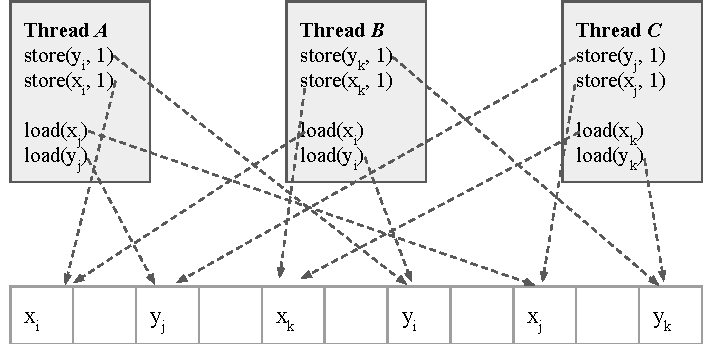
\includegraphics[width=.9\columnwidth]{images/parallel_strategy.pdf}
\caption{A visualization of how multiple threads coordinate to run parallel instances of litmus tests. }
\label{fig:parallel-ti}
\end{figure}

{\linespread{1.2}\selectfont
\begin{algorithm}
\small
\caption{Merging Test Environments}\label{alg:cap}
\begin{algorithmic}[1]
\State{// $t$: the mutant test to find a final environment for}
\State{// $E$: the set of environments that the mutant ran in}
\State{// $D$: the set of devices that ran the mutant (across the environments $E$)}
\State{// $r$: the reproducibility score target, $0 < r < 1$}
\State{// $b$: the maximum time the test should run, $ b > 0$}
\Function{MergeEnvironments}{$t$, $E$, $D$, $r$, $b$}
\State{$ceilingRate \gets \frac{\lceil -\log_{e}(1 - r) \rceil}{b}$}
\State{$e_r \gets $\O}
\State{$n_r \gets 0$}
\State{$minRate_r \gets \infty$}
\For{$e \in E$}
\State{$n_c \gets 0$}
\State{$minRate_c \gets \infty$}
\For{$d \in D$}
\State{// rate() calculates the death rate of $t$ on $d$ in $e$}
\State{$rate_c \gets \text{rate}(t, d, e)$}
\If{$rate_c \geq ceilingRate$}
\State{$n_c \gets n_c + 1$}
\EndIf
\If{$rate_c > 0$}
\State{$minRate_c \gets \min(minRate_c, rate_c)$}
\EndIf
\EndFor
\If{$n_c > n_r \lor (n_c == n_r \land minRate_c > minRate_r)$}
\State{$e_r \gets e$}
\State{$n_r \gets n_c$}
\State{$minRate_r \gets minRate_c$}
\EndIf
\EndFor
\State{\textbf{return} $e_r$}
\EndFunction
\end{algorithmic}
\label{alg:ceiling-rate}
\end{algorithm}
}

\begin{table}
\centering
\caption{The devices included in our study, along with how many compute units (CUs) they contain and a short name we will use throughout the text.}
\begin{tabular}{l l r l l l}
 \toprule
 \textbf{Vendor} & \textbf{Chip} & \textbf{CUs} & \textbf{Type}  & \textbf{Short}\\ %[0.5ex]
 & & & &\textbf{Name} \\
 \midrule
 NVIDIA & GeForce RTX 2080 & 64 & Discrete  & NVIDIA \\
 AMD & Radeon Pro 5500M & 24 & Discrete  & AMD\\
 Intel & Iris Plus Graphics & 48 & Integrated  & Intel\\
 Apple & M1 & 128 & Integrated  & M1\\
 \bottomrule
\end{tabular}
\label{table:gpus}
\end{table}

\begin{figure*}
\centering
\subfloat[Reversing \textit{po-loc} mutation scores (8 mutants)]{{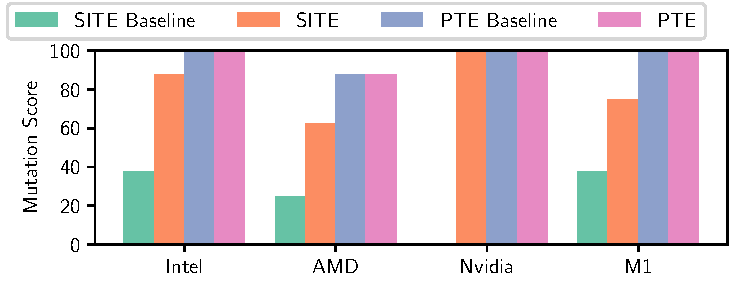
\includegraphics[width=0.5\columnwidth]{images/figure5a.pdf}\label{fig:5a}}}
\subfloat[Reversing \textit{po-loc} average mutant death rates]{{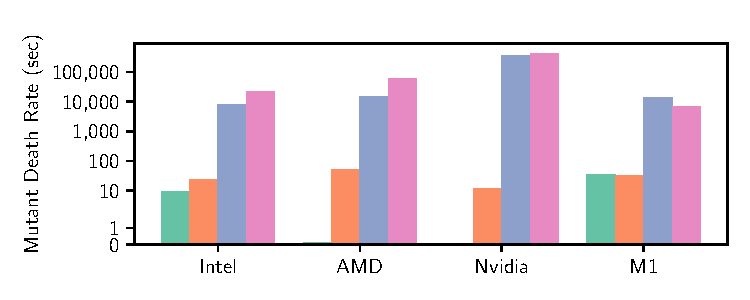
\includegraphics[width=0.5\columnwidth]{images/figure5b.pdf}\label{fig:5b}}} \\
\subfloat[Weakening \textit{po-loc} mutation scores (6 mutants)]{{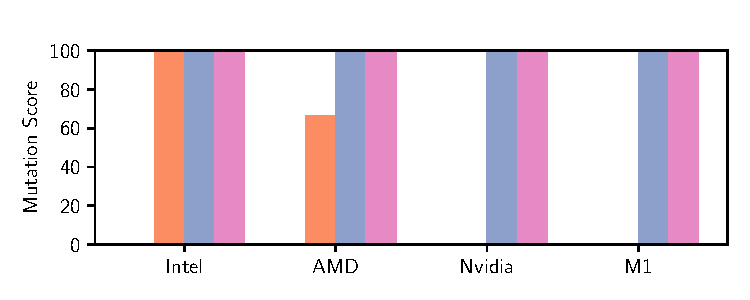
\includegraphics[width=.5\columnwidth]{images/figure5c.pdf}\label{fig:5c}}}
\subfloat[Weakening \textit{po-loc} average mutant death rates]{{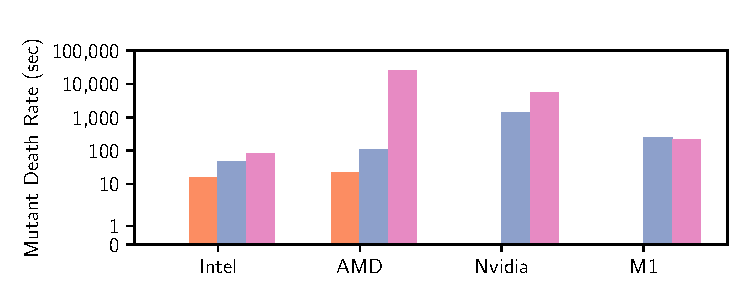
\includegraphics[width=0.5\columnwidth]{images/figure5d.pdf}\label{fig:5d}}} \\
\subfloat[Weakening \textit{sw} mutation scores (18 mutants)]{{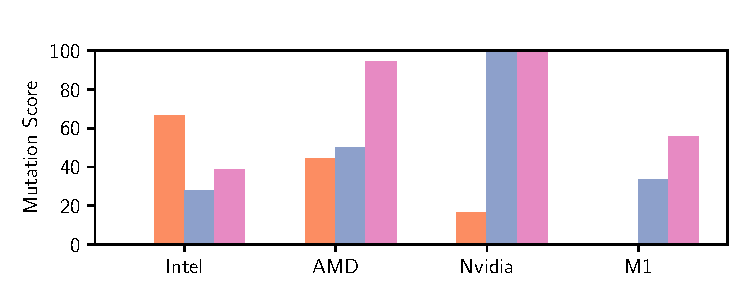
\includegraphics[width=0.5\columnwidth]{images/figure5e.pdf}\label{fig:5e}}}
\subfloat[Weakening \textit{sw} average mutant death rates]{{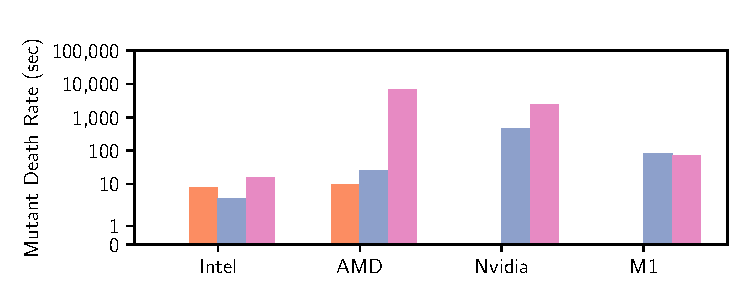
\includegraphics[width=0.5\columnwidth]{images/figure5f.pdf}\label{fig:5f}}} \\
\subfloat[All tests per device mutation scores (32 mutants)]{{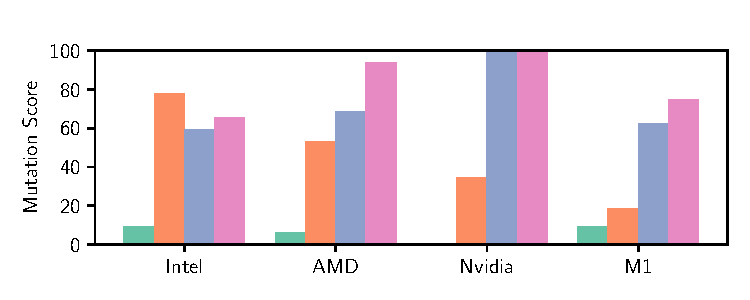
\includegraphics[width=0.5\columnwidth]{images/figure5g.pdf}\label{fig:5g}}}
\subfloat[All tests per device average mutant death rates]{{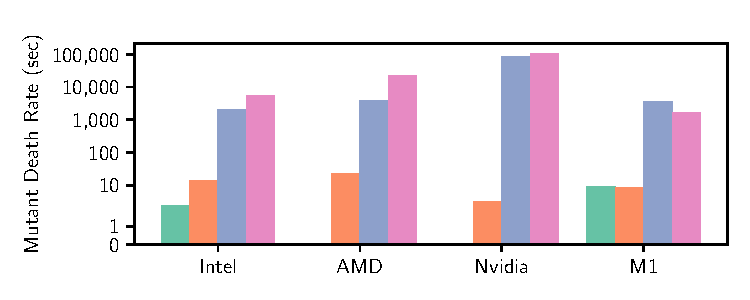
\includegraphics[width=0.5\columnwidth]{images/figure5h.pdf}\label{fig:5h}}} \\
\subfloat[All devices/tests mutation scores (128 mutants)]{{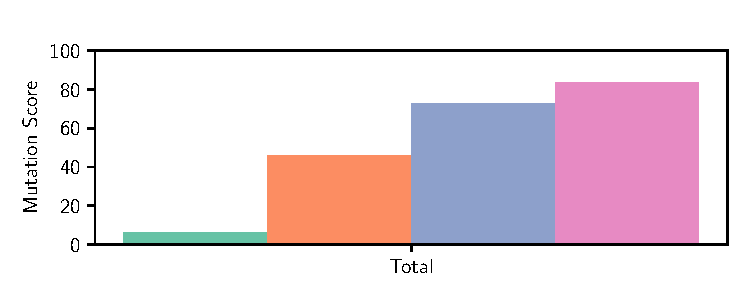
\includegraphics[width=0.5\columnwidth]{images/figure5i.pdf}\label{fig:5i}}}
\subfloat[All devices/tests average mutant death rates]{{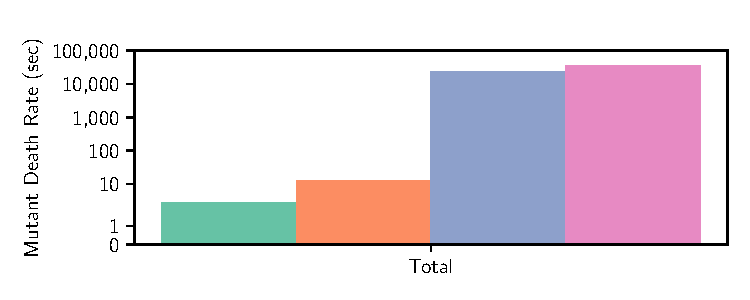
\includegraphics[width=0.5\columnwidth]{images/figure5j.pdf}\label{fig:5j}}}

\caption{Mutation scores and mutant death rates. \label{fig:total-scores} }
\end{figure*}

\begin{figure}
\hfill
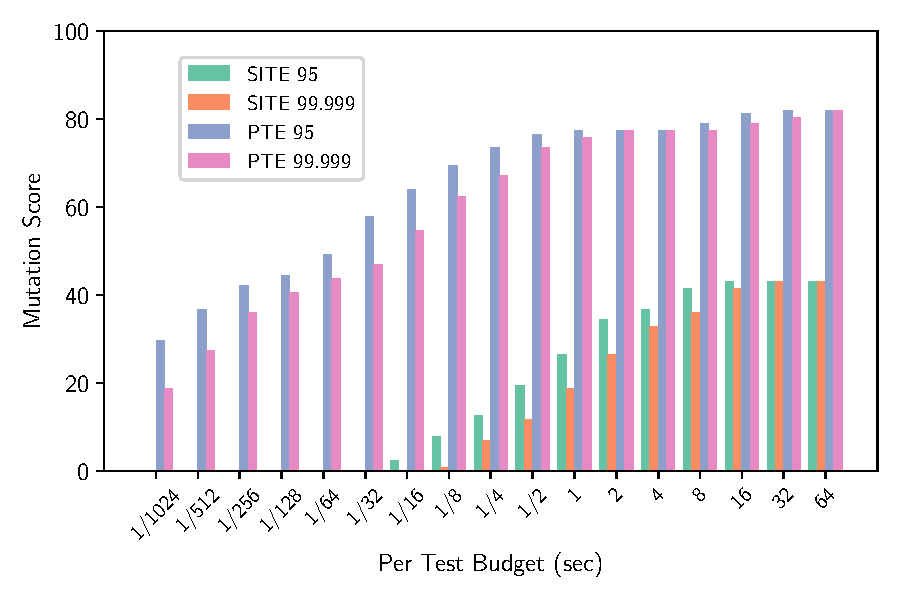
\includegraphics[width=\columnwidth]{images/merged.pdf}
\caption{Analyzing the impact of time budgets and reproducibility targets on mutation scores.}
\label{fig:budgets}
\end{figure}

\begin{table}
\centering
\caption{The Pearson Correlation Coefficient (PCC) between killing mutants and observing real bugs. Values for PCCs range from 0 to 1, and while it varies across domain, correlations greater than .8 are generally considered to be very strong.}
\begin{tabular}{l l l r}
 \toprule
 \textbf{Vendor} & \textbf{Failed Test} & \textbf{Mutant Type} & \textbf{PCC} \\
 \midrule
 Intel & CoRR & Reversing \textit{po-loc} & .996 \\
 AMD & MP-relacq & Weakening \textit{sw} & .967 \\
 NVIDIA & MP-CO & Weakening \textit{po-loc} & .893 \\
 \bottomrule
\end{tabular}
\label{table:corr-analysis}
\end{table}
